\documentclass[preview]{standalone}

\usepackage{amsmath}
\usepackage{amssymb}
\usepackage{stellar}
\usepackage{bettelini}
\usepackage{wrapfig}

\hypersetup{
    colorlinks=true,
    linkcolor=black,
    urlcolor=blue,
    pdftitle={Biologia},
    pdfpagemode=FullScreen,
}

\begin{document}

\id{biologia-sistema-respiratorio}
\genpage

\section{Trasporto dei gas}

\begin{snippet}{aec421b4-c0d6-4f27-a994-d3ba7807c83d}
    \begin{wrapfigure}{l}{0.525\textwidth}
        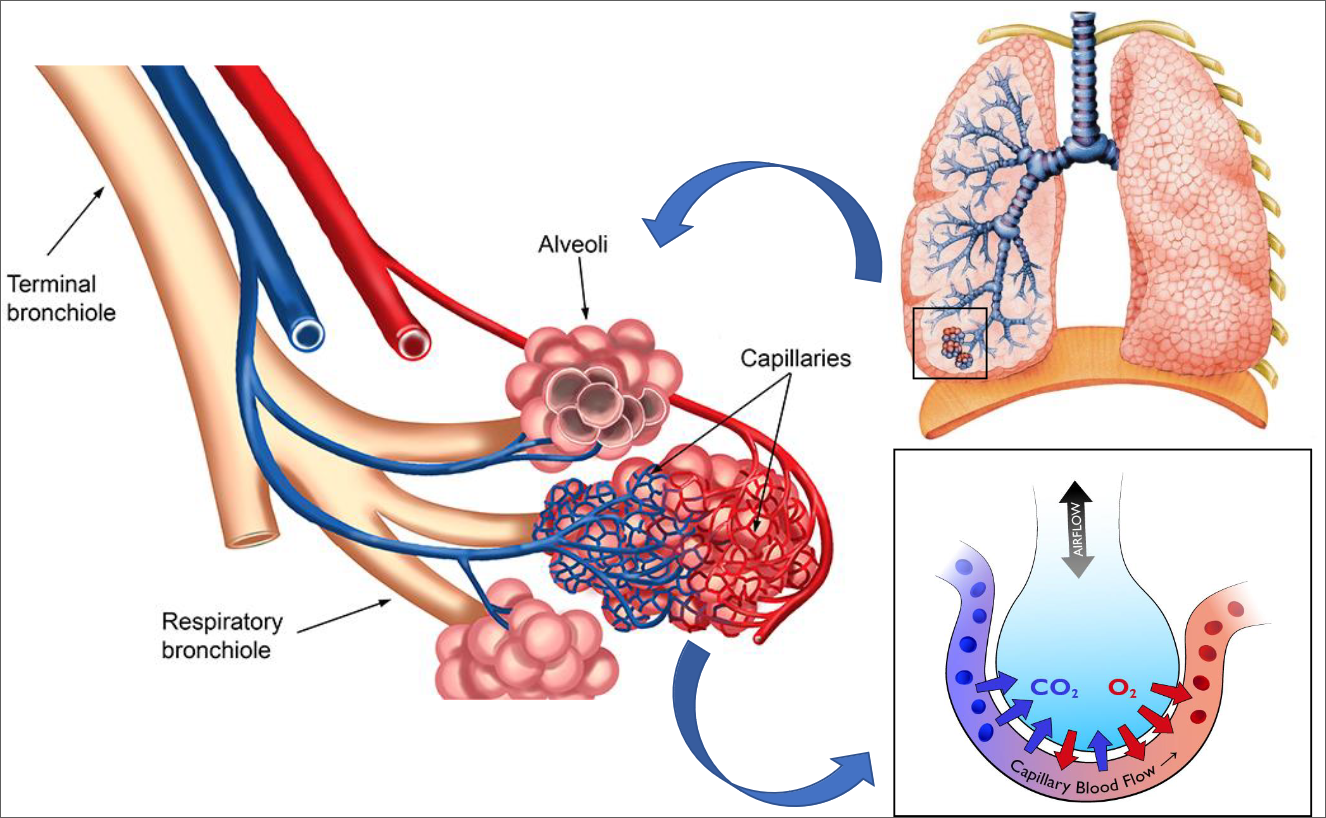
\includegraphics[width=0.5\textwidth]{./resources/gas_transport.png}
    \end{wrapfigure}
    
    Gli scambi avvengono fra gli alveoli, dove avviene l'incontro fra il sistema
    circolatorio e quello respiratorio.
    I gas si muovono per diffusione semplice, e quindi passano fra i fosfolipidi (per gradiente di concentrazione).
    Non è quindi possibile controllare la diffusione dei gas.
    
    Una molecola di ossigeno deve trasversare 5 membrane per legare con l'emoglobina.
    \wrapfill
\end{snippet}

\begin{snippetdefinition}{pressione-parziale-definition}{Pressione parziale}
    La \textit{pressione parziale} (mmHg) corrisponde alla concentrazione di gas.
\end{snippetdefinition}

\begin{snippet}{f1e5ee30-6674-4190-9a5e-cf306c8aab09}
    In tutti i vasi rossi la concentrazione di ossigeno è 100 mmHg, mentre in quelli blu è 40 mmHg.
    \\
    Nell'alveolo il gas rispecchia quello nell'ambiente circostante.
    La concentrazione della cellula nei capillari è più bassa (40 o meno se sotto sforzo).
\end{snippet}

\section{Modalità di trasporto dell'ossigeno}

\begin{snippet}{trasporto-ossigeno}
    \vspace{-0.5cm}
    \begin{enumerate}
        \item Alla pressione parziale di pO\({}_2=100\) mmHG, presente nell'aria alveolare,
        solo 0.3 ml di O\({}_2\) (1.5\%) si sciolgono ogni 100 ml di sangue.
        \item La maggior parte dell'ossigeno (98.5\%), viene trasportato legato all'emoglobina.
        \item Per ogni globulo rosso ci sono 260 milioni di emoglobine.
    \end{enumerate}
\end{snippet}

\section{Modalità di trasporto dell'anidride carbonica}

\begin{snippet}{trasporto-co2}
    \vspace{-0.5cm}
    \begin{enumerate}
        \item Parte del CO\({}_2\) (5\%), viene trasportato disciolto nel plasma.
        \item Un'altra parte (5\%) si lega all'emoglobina.
        \item La maggior parte del CO\({}_2\) nel sangue (90\%) è trasportato nel plasma come ione bicarbonato. 
    \end{enumerate}
    
    Nel sangue dobbiamo avere una pH stabile, ma diossido di carbonio e acqua
    si legano formando acido carbonico. Il globulo rosso spacca quindi questo acido,
    tenendo l'idronio e rilasciando nel sangue solo lo ione bicarbonato.
    Il bicarbonato torna CO2, il quale fuoriesce nei polmoni.
    Ogni emoglobina può legare con 4 ossigeni.
\end{snippet}

\section{Curva di dissociazione dell'emoglobina}

\includesnpt[width=65\%|src=/snippet/static/emoglobina.png]{centered-img}

\begin{snippet}{dissociazione-emoglobina}
    L'emoglobina lega con l'ossigeno in maniera non lineare.
    La sua affinità nel legare con l'ossigeno dipende dalla concentrazione.
    
    All'aumentare della PO2 la quantità di O2 che si lega all'Hb
    prima aumenta rapidamente, poi tende a stabilizzarsi quando la saturazione si avvicina al 100\%.
    Come mostra la tabella, alle normali pressioni parziali nelle
    arterie e nelle vene sistemiche, a riposo, la percentuale di saturazione dell'Hb varia solo del 25\% circa.
    
    Più le emoglobine sono legate con l'ossigeno, più è difficile che l'ossigeno si leghi con quelle rimanente,
    e di conseguenza l'affinità dell'emoglobina è maggiore (vicino all'alveolo).
    
    Vicino ai polmoni l'affinità è 100\%, mentre ai tessuri (40 mmHG), l'affinità è 75\%, per
    cui 3/4 ossigeni per emoglobina.
    
    Per sopravvivere ad un altitudine maggiore, dove l'ossigeno arriva ad una concentrazione del
    75\%, l'affinità è comunque quasi 100\%. Di conseguenza, in alta montagna le emoglobine sono comunque
    piene anche se la concentrazione dell'aria è minore.
\end{snippet}

\end{document}